\begin{figure}[h!]
	\centering
	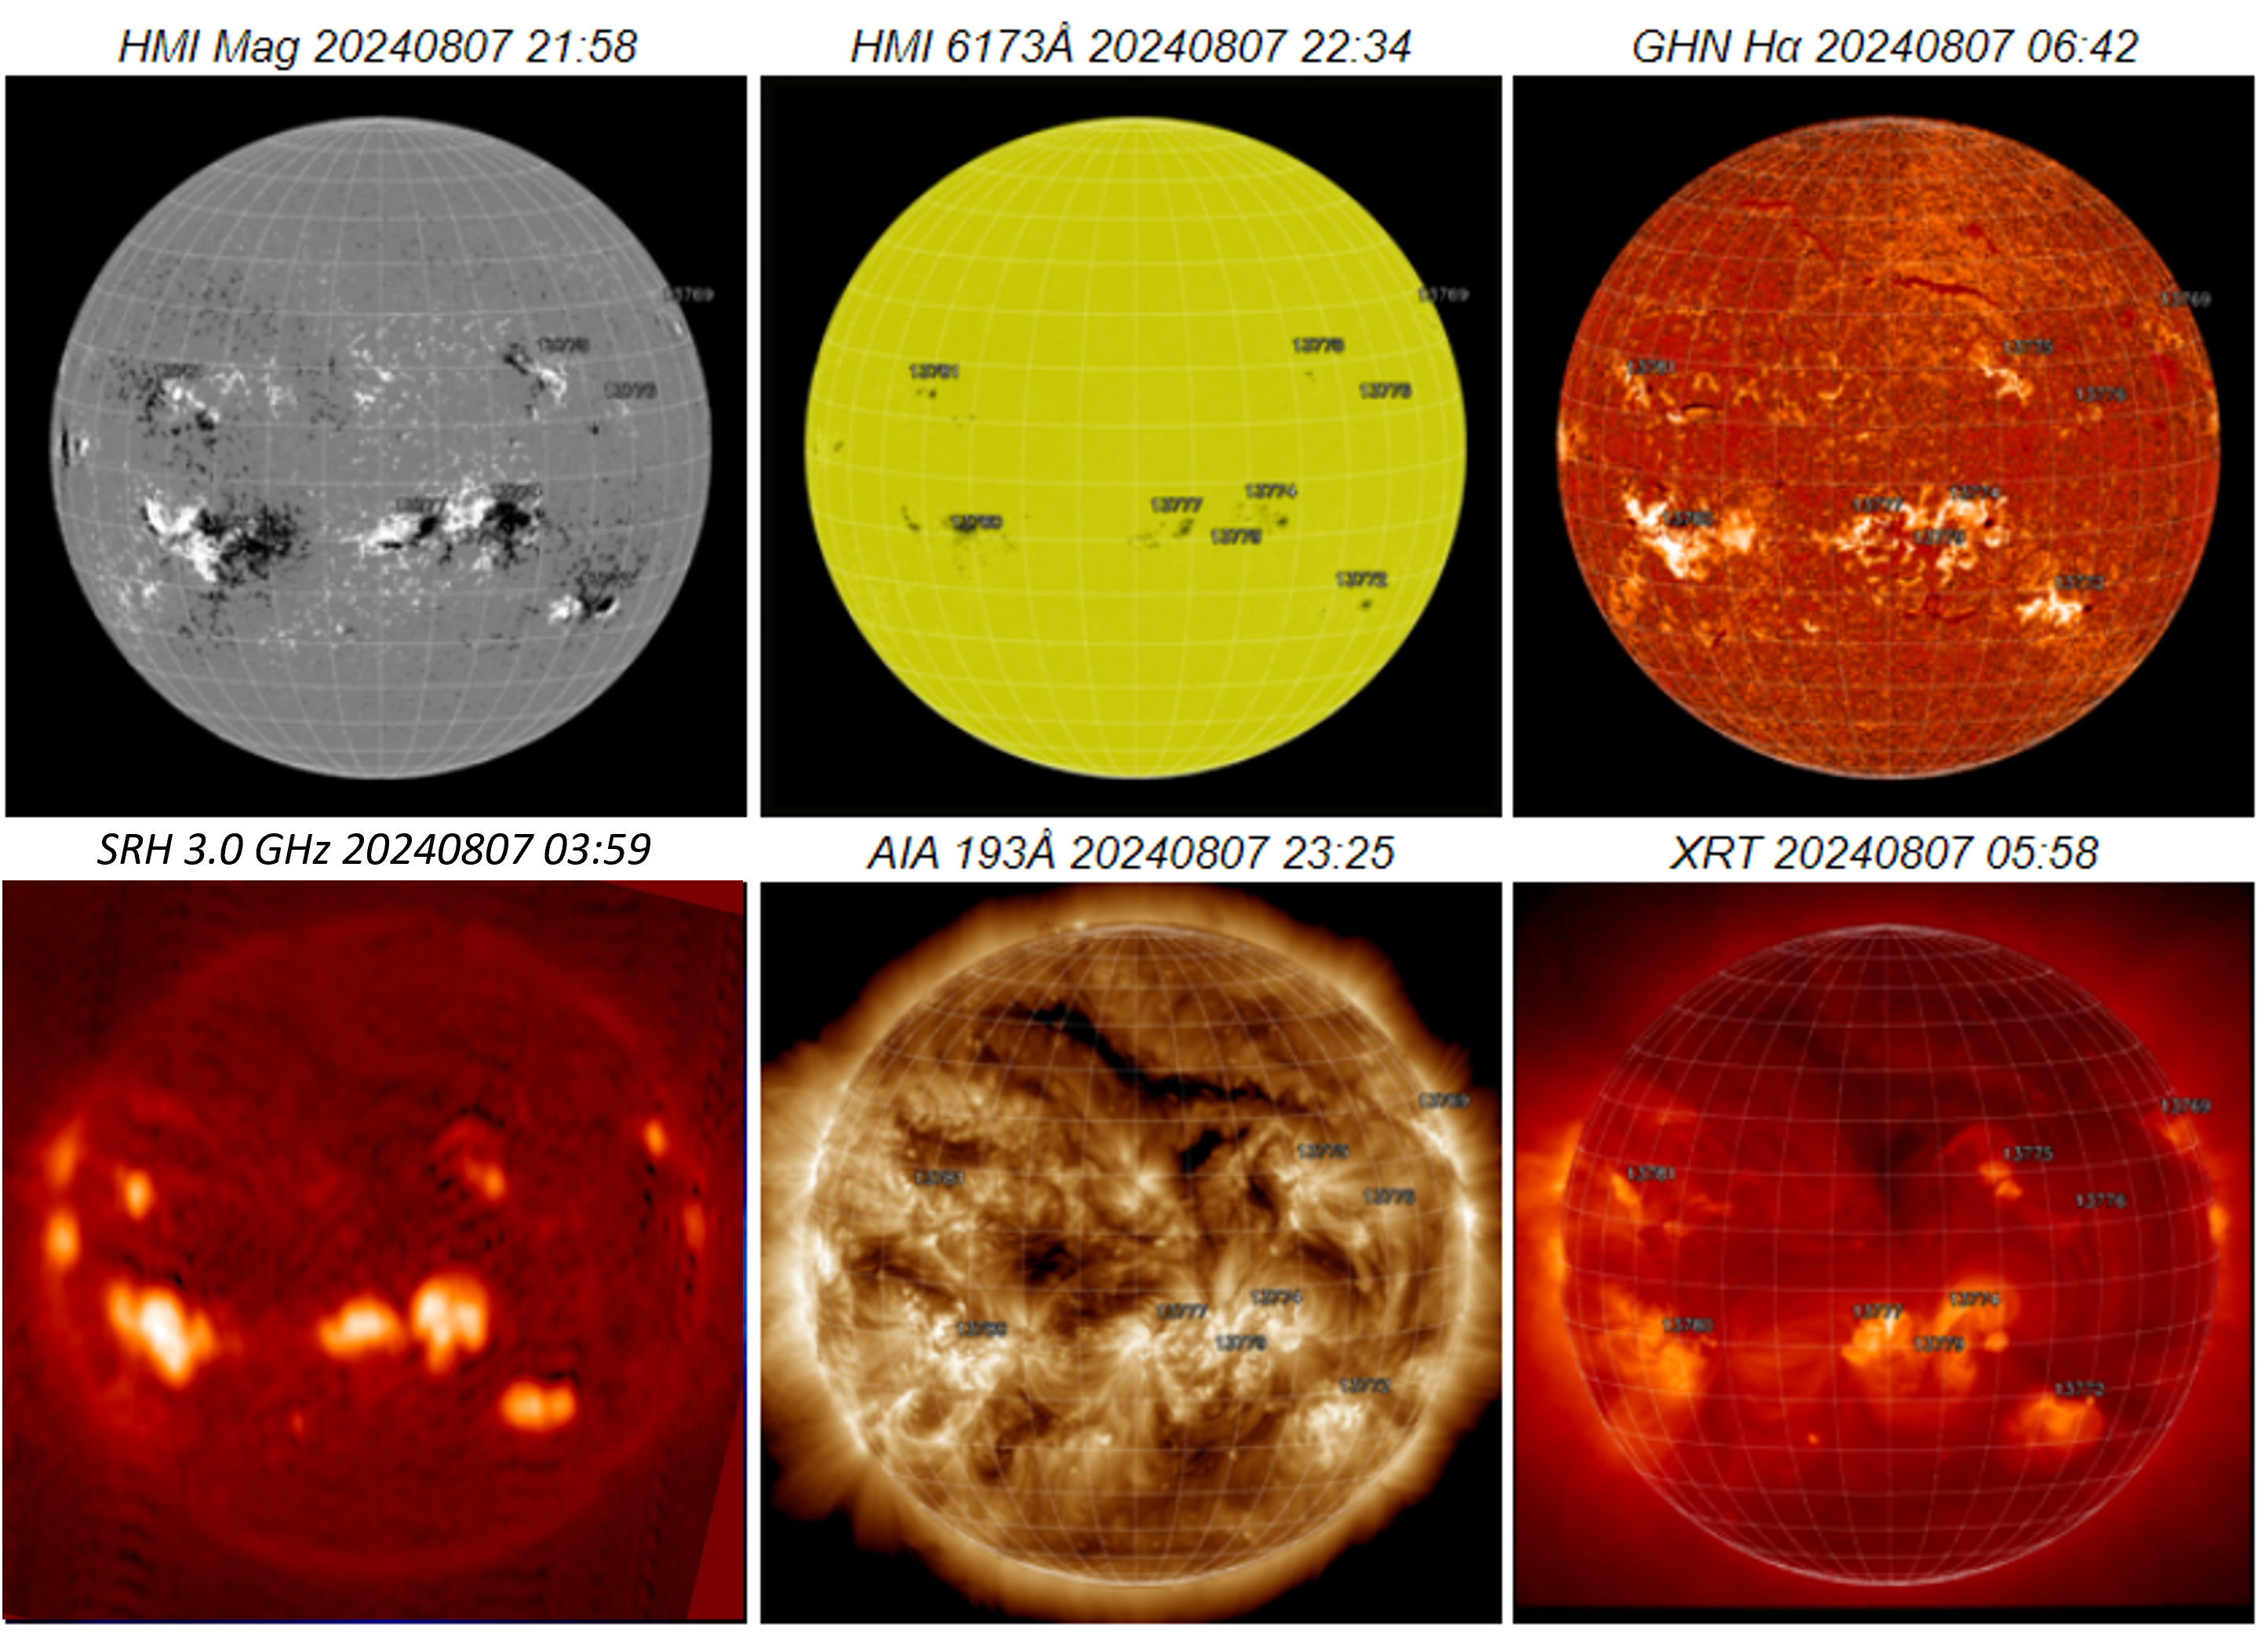
\includegraphics[width=1\linewidth]{images/grechnev1.png}
	\caption{Изображения солнечного диска 7 августа 2024 года в разных длинах волн}
	\label{grechnev1}
\end{figure}

Обратимся к \cref{grechnev1}. Между изображениями есть определенные сходства, но тем не менее они довольно сильно отличаются друг от друга, и разобраться с запечатленными на снимках в разных спектральных диапазонах процессами обычно довольно проблематично. Часто это осложняется еще и скоротечностью данных процессов.
Для облегчения этой задачи можно использовать совместное использование изображений разных диапазонов, что позволяет более полно восстановить картину происходящего события, установить последовательность явлений и выявить причинно-следственные связи между ними, структуру изучаемого объекта на разных высотах, а также выяснить физические условия в изучаемых объектах и их взаимосвязи.

Совместное использование данных может быть также полезно с точки зрения подтверждения или опровержения догадок, сделанных на основе изучения данных в определенном частотном диапазоне.

\subsection{Одномерные массивы данных (обычно, временные ряды)}
	
В первую очередь, стоит обратить внимание, к какой системе отсчета времени привязан массив данных. Это может быть, например, всемирное время $UT$, определяемое на основе наблюдений за вращением Земли, международное атомное время $TAI$, определяемое через период излучения атома цезия-133, или всемирное координированное время $UTC$, которое учитывает колебания скорости вращения Земли и регулирует эти неточности с помощью дополнительных "<високосных"> секунд, что делает $UTC$ близким к $UT$, но с точностью атомных часов.

\begin{figure}[h!]
	\centering
	\includegraphics[width=0.55\linewidth]{images/grechnev2.png}
	\caption{Разница между $UT$ и $UTC$}
	\label{grechnev2}
\end{figure}

Разница между $UT$/$UTC$ и $TAI$ составляет, на данный момент, $37$ секунд, что иногда может быть очень существенно. И хоть $TAI$ используется довольно редко, предпочтительнее использовать при анализе одномерных временных рядов зависимость величины не от номера отсчета, а от временной отметки, когда данные были получены. Это поможет избежать ошибок из-за:
\begin{enumerate}
	\item неравномерных отсчетов
	\item записей с пропусками
	\item сбоев записи времени
	\item использования данных с разными шкалами времени
\end{enumerate}
В IDL это можно реализовать путем использования команды:
\begin{python}
	plot, x, y
\end{python}
Или при использовании нескольких графиков с разными шкалами:
\begin{python}
	plot, time1, y1
	oplot, time2, y2
\end{python}
В Python для этого можно использовать:
\begin{python}
	import matplotlib.pyplot as plt
	def format_seconds(x, pos):
	hours = int(x // 3600)
	minutes = int((x % 3600) // 60)
	seconds = int(x % 60)
	return f"{hours:02d}:
	{minutes:02d}:
	{seconds:02d}"
	plt.plot(time, data)
	ax.xaxis.set_major_formatter(
	FuncFormatter(format_seconds))
\end{python}

\begin{figure}[h!]
	\centering
	\includegraphics[width=0.65\linewidth]{images/grechnev3.png}
	\caption{Пример правильного отображения данных с пропусками}
	\label{grechnev3}
\end{figure}

Подобный подход позволит создать интерактивную ось времени, при манипуляции с которой (приближении и т. п.) метки останутся верными

Также стоит обратить внимание на валидацию данных и их фильтрацию. К типичным методам можно отнести:
\begin{enumerate}
	\item сглаживание скользящим усреднением: $[1, 4, 100] \Rightarrow 35$
	\item медианное сглаживание: $[1, 4, 100] \Rightarrow 4$\\
	(может быть полезно для оценки стационарного уровня при анализе всплеска излучения)
	\item суммирование отсчетов\\
	(данный подход нужно использовать с осторожностью из-за его фазочувствительности)
	\item Фурье-фильтрация\\
	(разложение исходного сигнала на гармонические составляющие для выделения шумов)
	\item полиномиальная аппроксимация\\
	(повышение порядка полинома повышает точность, но снижает устойчивость)
	\item выделение огибающих и трендов (см. \cref{grechnev4})\\
	(иногда можно заменить аппроксимацией точек минимумов в массиве данных каким-либо способом)
\end{enumerate}

\begin{figure}[h!]
	\centering
	\includegraphics[width=0.65\linewidth]{images/grechnev4.png}
	\caption{Пример использования огибающих}
	\label{grechnev4}
\end{figure}

\subsection{Двумерные массивы данных (обычно, изображения)}

\begin{enumerate}
	\item \textsf{Отображение}
	
	При отображении данных важно правильно подобрать шкалу яркости. Она может быть линейной, степенной, логарифмической, определена какой-то сложной функцией (например, $asinh$), или вообще иметь разные масштабы изменения для разных диапазонов значений (пример -\\ \texttt{matplotlib.colors.TwoSlopeNorm(vcenter, vmin=None, vmax=None)}, что может быть полезно при анализе изображений солнечных вспышек с большим динамическим диапазоном)
	
	\begin{figure}[h!]
		\centering
		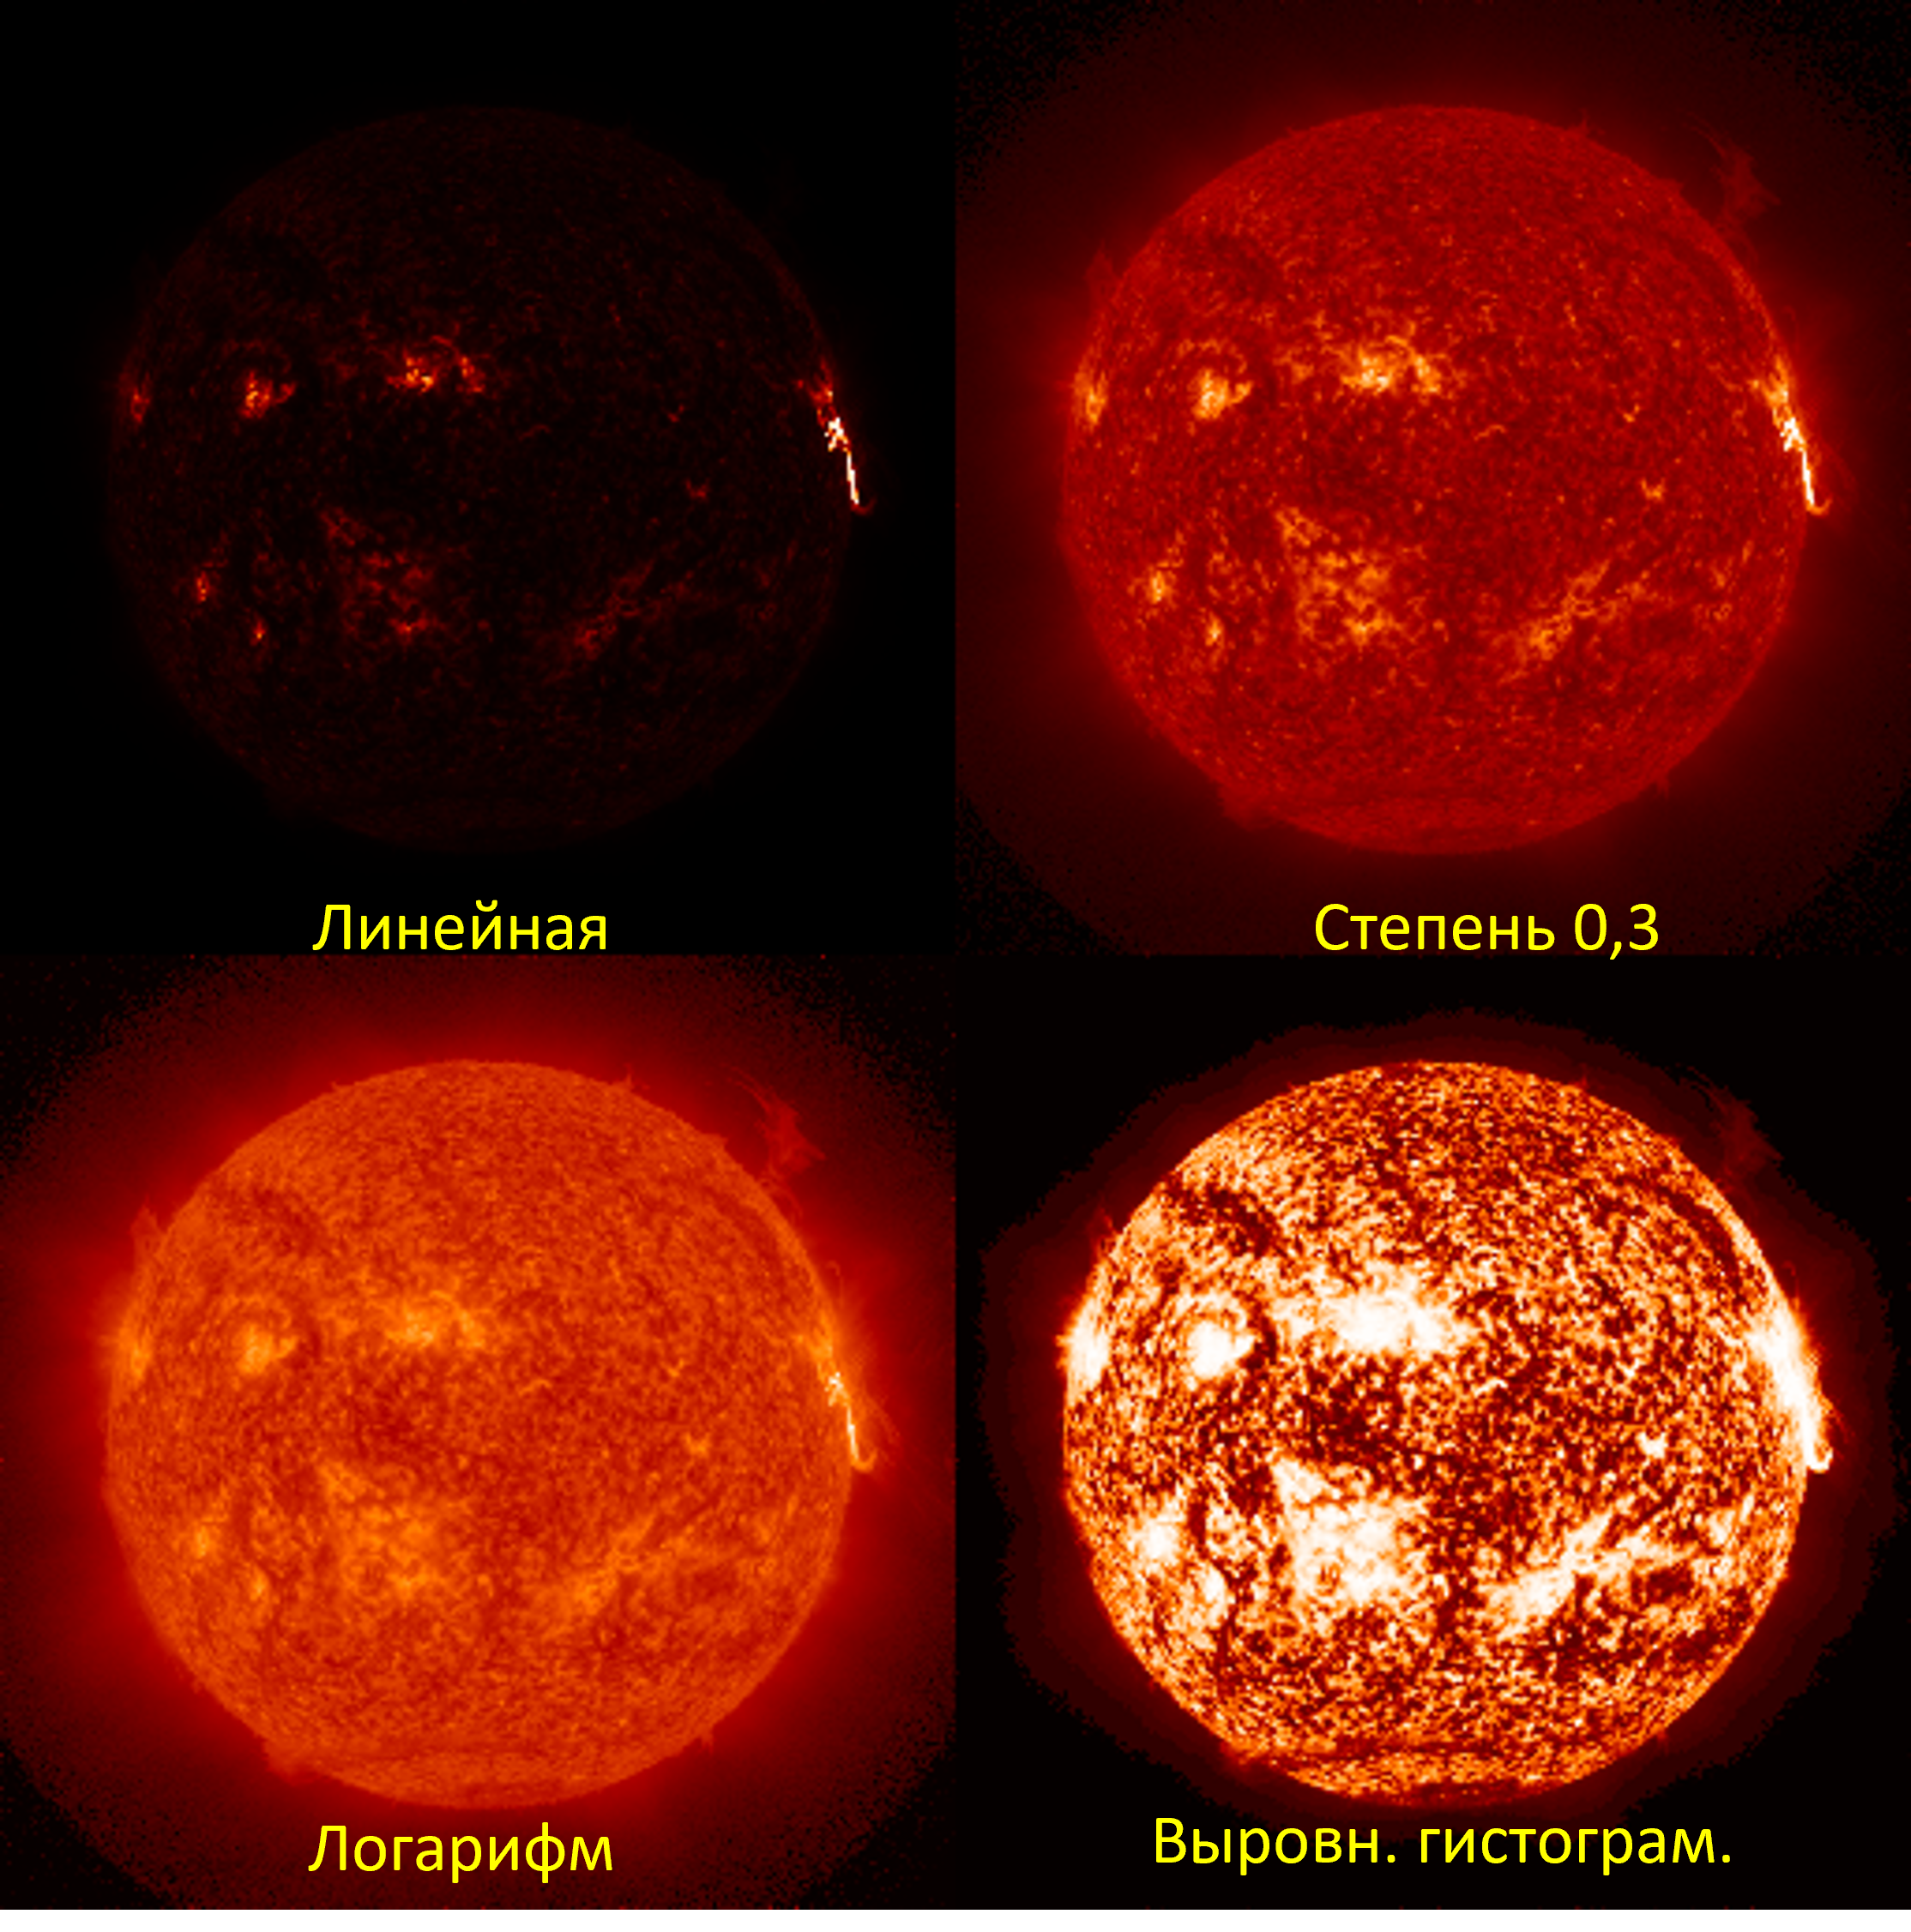
\includegraphics[width=0.75\linewidth]{images/grechnev5.png}
		\caption{Пример использования различных шкал яркости. Для случая линейной шкалы выполнено ограничение по порогу}
		\label{grechnev5}
	\end{figure}
	
	\begin{figure}[h!]
		\centering
		\includegraphics[width=0.7\linewidth]{images/grechnev6.png}
		\caption{Наглядная демонстрация принципа работы нормировки \texttt{TwoSlopeNorm}}
		\label{grechnev6}
	\end{figure}
	
	Также довольно удобным инструментом анализа изображений являются контуры уровня (см. \cref{grechnev7})
	
	\begin{figure}[h!]
		\centering
		\includegraphics[width=0.7\linewidth]{images/grechnev7.png}
		\caption{А - использование контуров при анализе изображений, Б - "<Раскраска пятен">}
		\label{grechnev7}
	\end{figure}
	
	\item \textsf{Подавление фона и выделение изменений}
	
	Для этой цели широко используется разностные изображения. Их есть два вида: бегущие (последовательные) разности (\textit{Running Difference} - RD) и фиксированные разности (\textit{Fixed Difference} - \textit{FD})
	
	\begin{figure}[h!]
		\centering
		\includegraphics[width=0.7\linewidth]{images/grechnev8.png}
		\caption{Использование разностных изображений. Видно потемнение области }
		\label{grechnev8}
	\end{figure}		
\end{enumerate}